
%%
%% Historical context
%%

\begin{frame}{Historical Context}

\begin{itemize}
\item Every 7th-degree can be algebraically reduced to
  $x^{7}+ax^{3}+bx^{2}+cx+1=0$ \textcolor{citations}{(Tschirnhaus, 1683)}
  \begin{itemize}
  \item Solving this means finding the three-variable function that maps
    $a,b,c$ to $x$
  \end{itemize}
\item \textcolor{citations}{Hilbert's 13th (1900, 1902)}:
  Can this function be expressed as the composition of a finite number
  of two-variable functions?
\item \textcolor{citations}{Kolmogorov (1956)}: Every continuous multi-variable function
  can be expressed as the composition of a finite number of
  three-variable functions
\item \textcolor{citations}{Arnold (1957)}: Only two-variable functions are really needed
\item \textcolor{citations}{Kolmogorov (1957)}: Actually, the only two-variable function
  needed is addition
  \begin{itemize}
  \item A generalization of Hilbert's question,
    except that the univariate functions are not necessarily algebraic
  \end{itemize}
\end{itemize}

\end{frame}



\begin{frame}{Kolmogorov-Arnold Representation Theorem}

\begin{columns}

  \begin{column}{6cm}
  \begin{itemize}
  \item Every multi-variate continuous function $f$ can be
    written using only univariate functions and addition:
    $$
    f(x_{i=1..n}) = \sum_{q=0}^{2n}\phi_q\left(\sum_{p=1}^n\psi_{q,p}(x_p)\right)
    $$
  \item In other words, addition is the only real multi-variate function,
    everything else is syntactic sugar
  \end{itemize}
  \end{column}

  \begin{column}{7cm}
  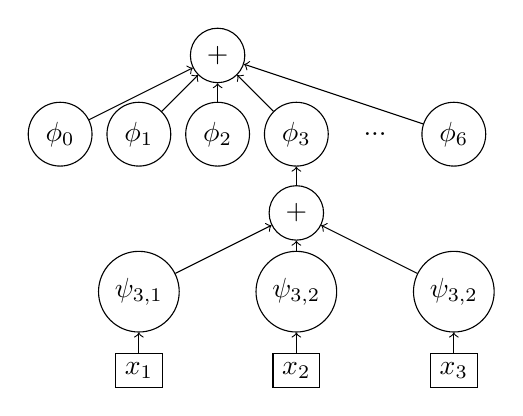
\begin{tikzpicture}
    \node[shape=circle,draw=black] (sum) at (0,0) {+};

    \node[shape=circle,draw=black] (F0) at (-2,-1) {$\phi_0$};
    \path [->] (F0) edge (sum);
    \node[shape=circle,draw=black] (F1) at (-1,-1) {$\phi_1$};
    \path [->] (F1) edge (sum);
    \node[shape=circle,draw=black] (F2) at (0,-1) {$\phi_2$};
    \path [->] (F2) edge (sum);
    \node[shape=circle,draw=black] (F3) at (1,-1) {$\phi_3$};
    \path [->] (F3) edge (sum);
    \node[shape=rectangle,draw=white] (dots) at (2,-1) {$...$};
    \node[shape=circle,draw=black] (F6) at (3,-1) {$\phi_6$};
    \path [->] (F6) edge (sum);

    \node[shape=circle,draw=black] (sum2) at (1,-2) {+};
    \path [->] (sum2) edge (F3);

    \node[shape=circle,draw=black] (f31) at (-1,-3) {$\psi_{3,1}$};
    \path [->] (f31) edge (sum2);
    \node[shape=circle,draw=black] (f32) at (1,-3) {$\psi_{3,2}$};
    \path [->] (f32) edge (sum2);
    \node[shape=circle,draw=black] (f33) at (3,-3) {$\psi_{3,2}$};
    \path [->] (f33) edge (sum2);

    \node[shape=rectangle,draw=black] (x1) at (-1,-4) {$x_1$};
    \path [->] (x1) edge (f31);
    \node[shape=rectangle,draw=black] (x2) at (1,-4) {$x_2$};
    \path [->] (x2) edge (f32);
    \node[shape=rectangle,draw=black] (x3) at (3,-4) {$x_3$};
    \path [->] (x3) edge (f33);

  \end{tikzpicture}
  \end{column}

\end{columns}

\end{frame}



\begin{frame}{Sprecher Formulation}

\begin{columns}

  \begin{column}{6cm}
  \textcolor{citations}{Sprecher (1972)} gives an alternative formulation with a single function
  at the lower layer:
  $$
  f(x_{i=1..n}) = \sum_{q=0}^{2n}\phi_q\left(\sum_{p=1}^n\lambda^{p-1}\psi(x_p+q\cdot\epsilon)+q\right)
  $$
  where $\phi_q$ are continuous,
  $\psi$ is monotonically increasing and Lipschitz-1 continuous,
  $\lambda$ and $\psi$ depend only on $n$ and not on $f$,
  and $\epsilon$ is any non-zero constant
  \end{column}

  \begin{column}{7cm}
  \input{contents/kat_sprecher}
  \end{column}

\end{columns}

\end{frame}



\begin{frame}{Some Intuitions}

\begin{columns}

  \begin{column}{6cm}
  \begin{itemize}
  \item Sprecher uses powers of $\lambda$ but other non-linear
    sequences also work
  \item Feels like multiple values in the unit interval are
    \quotes{packed} into a single value in $\mathcal{R}$
  \item Think how addition of powers of 10 packs single-digit
    numbers into multiple-digit numbers in a reversible way, $42$ can
    only be the sum of the powers of $4$ and $2$.
  \end{itemize}
  \end{column}

  \begin{column}{7cm}
  \input{contents/kat_sprecher}
  \end{column}

\end{columns}

\end{frame}



\begin{frame}{Some Intuitions}

\begin{columns}

  \begin{column}{6cm}
  \begin{itemize}
  \item $\psi$ has many `intervals' and translating by $q\cdot\epsilon$
    lands $x_i$ into the right interval
    \begin{itemize}
    \item hacks the multiple $\psi_i$ functions into one that
      behaves differently in each interval
    \end{itemize}
  \item The lower level `packs' the effect of~$f$ on~$x_i$ for
    different values of the other inputs $x_{j\neq i}$
  \item The $\phi$ functions can now \quotes{decode} the sums into
    the original values and calculate the result.
  \end{itemize}
  \end{column}

  \begin{column}{7cm}
  \input{contents/kat_sprecher}
  \end{column}

\end{columns}

\end{frame}


\begin{frame}{Proof Sketch}

The actual proof is between $E^n$ and $E^{n-1}$, which gives inductively
that a function in $E^n$ can be represented with functions in $E$.

To allow for nice figures, we will show that for any $f:E^2\rightarrow\mathcal{R}$
there are $\phi_{0..4}:\mathcal{R}\rightarrow\mathcal{R}$
and $\psi_{0..4,1..2}:E\rightarrow\mathcal{R}$ such that:
$$
f(x_1,x_2)=\sum_{q=0}^4\phi_q\left(\psi_{q,1}\left(x_1\right)+\psi_{q,2}\left(x_2\right)\right)
$$

The proof proceeds in three steps:
%
\begin{itemize}
\item Break the input range into non-overlapping intervals with gaps
\item Construct the inner functions $\psi$
\item Construct the outer functions $\phi$
\end{itemize}
\end{frame}



\begin{frame}{Proof Sketch Step 2: Construct the inner functions}

\begin{columns}

  \begin{column}{7cm}

  For given $k$ non-overlapping intervals, it is always possible to
  construct a series of constants $\lambda_i$ such that:

  $$
  \lambda_i < \lambda_{i+1} \leq \lambda_i + \frac{1}{2^k}
  $$

  and a function $\psi_1$ mapping inputs from the
  $A_{k,1}^q$ intervals to the corresponding $\lambda$ intervals.

  \vskip 1em

  Any continuous function will do, but let's say it's a step function
  with linear connections across gaps, so that it's continuous and
  monotonic increasing.

  \end{column}

  \begin{column}{6.5cm}
  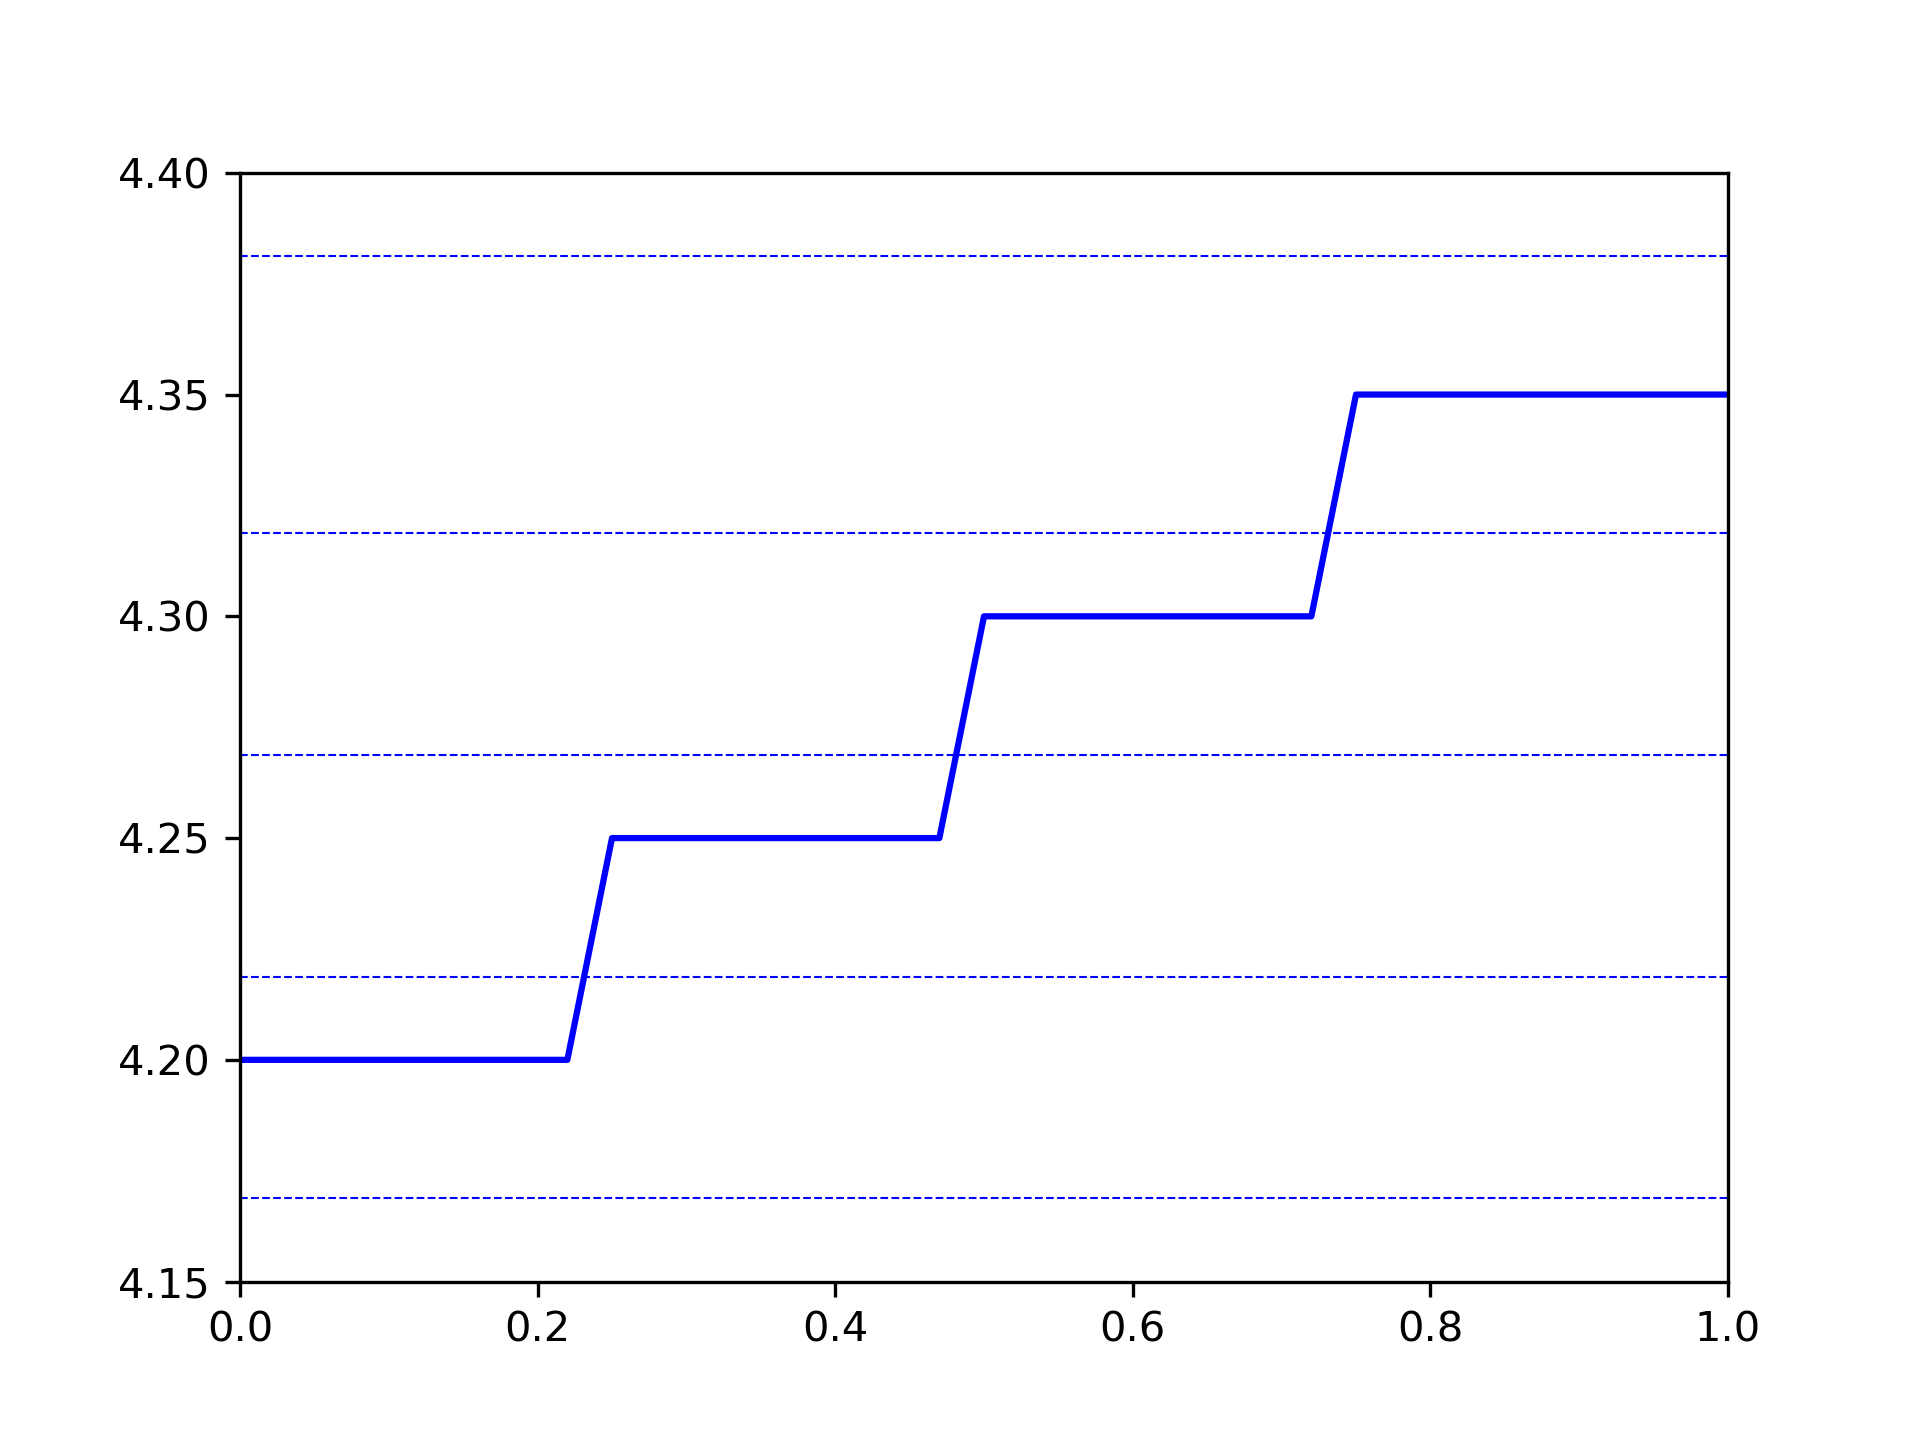
\includegraphics[width=6cm]{contents/images/kat_psi1}

  For $k=4$, four non-overlapping intervals and
  the corresponding `lanes' defined by the $\lambda$ series.
  \end{column}

\end{columns}

\end{frame}



\begin{frame}{Proof Sketch Step 2: Construct the inner functions}

\begin{columns}

  \begin{column}{7cm}
  Construct a similar series for the second dimension; Then... Add.
  \vskip 1em
  There are many solutions, but \textcolor{citations}{Sprecher's (1972)} formulation gives us
  something we can visualize:
  \vskip 1em
  A grid of non-overlapping \quotes{platforms}, linearly connected at the
  gaps, all having different $z$, so that each $z$ maps to exactly
  one $S_k$ or to a gap.
  \end{column}

  \begin{column}{6.5cm}
  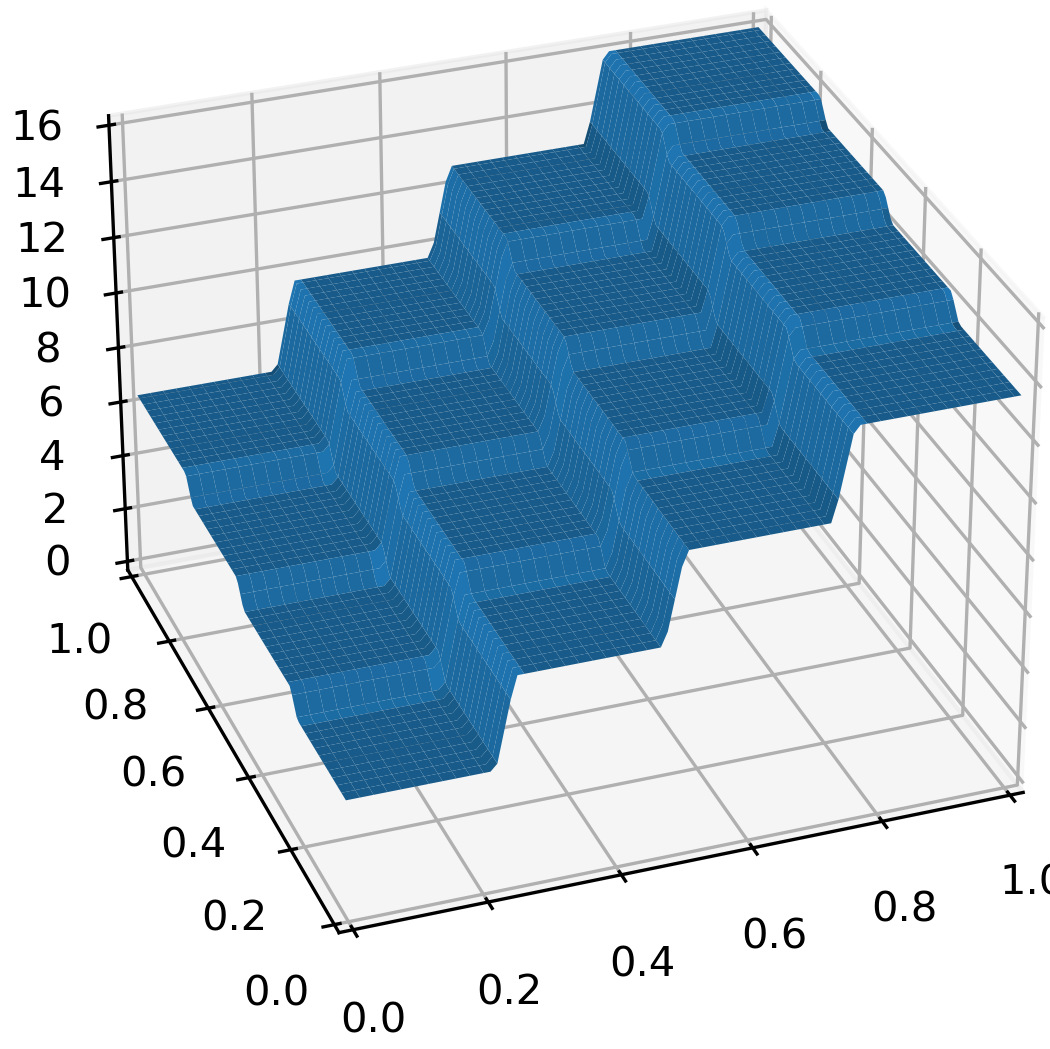
\includegraphics[width=6cm]{contents/images/kat_psi3}
  \end{column}

\end{columns}

\end{frame}



\begin{frame}{Proof Sketch Step 2: Construct the inner functions}

We repeat all the above for to create $2n+1$ different
systems of `platforms', one for each upper function.

\vskip 1em

Step 1 constructed the non-overlapping intervals and \textit{also}
\vspace{0.5em}
\begin{itemize}
\item includes the proof that these intervals can always be constructed so that every point in $E^2$ is covered
  by at least one non-gap area of one of these systems of `platforms'
\item \textit{Intuition:} Do not align the gaps  
\end{itemize}

\vskip 1em

So:
\vspace{0.5em}
\begin{itemize}
\item For each of the $2n+1$ outer functions,
  we have created the inner functions that map from \emph{some} values of
  $\psi_1(x_1)+\psi_2(x_2)$ to a platform
\item Some other values might be over a gap.
\item \textit{But:} There is no value that is over a gap in \emph{all} systems of
  platforms
\end{itemize}

\end{frame}



\begin{frame}{Proof Sketch Step 3: Construct the outer functions}

All the pieces are now in place:
\vspace{0.5em}
\begin{itemize}
\item We have an `index' from $\psi_1(x_1)+\psi_2(x_2)$ to squares
  restricting the possible values of $x_1,x_2$. The size of the
  squares gets smaller as $k$ gets larger. \vspace{0.4em}
\item We can construct a function $f_k$ that simply `memorizes' how to
  approximate the value of the original $f$:
  \vspace{0.3em}
  \begin{itemize}
  \item all pairs in the unit square are covered
  \item $f_k$ knows the neighbourhood of the $x_1,x_2$ values despite the fact
    that it only sees sums
  \item $f_k$ can estimate $f$ with some error bounded by an
    expression denominated by $k$
  \end{itemize} \vspace{0.4em}
\item As the number of intervals $k$ increases, the error
  decreases. At the limit, there is no error.
\end{itemize}

\vskip 0.8em

\begin{center}
\textcolor{blue!50!black}{%
  Unlike the $\psi$ functions, we have no intuitions whatsoever
  about what the $\phi$ functions look like or how to construct them.
}
\end{center}

\end{frame}



\begin{frame}{Some Thoughts and Intuitions}

\begin{itemize}
\item The theorem premises that $x_i$ are in the unit interval---this
  is needed for some of the constructions in the proof and is not a
  real restriction \vspace{0.5em}
\item The theorem proves the existence of the $\phi$ and $\psi$
  functions, does not tell you how to construct them \vspace{0.5em}
\item We know very little about $\phi$ (continuous) and slightly more
  (but still little) about $\psi$ (monotonic increasing and
  Lip-1 continuous) \vspace{0.5em}
\item It is unlikely that these functions can be defined by a
  neat-looking closed formula
\end{itemize}

\end{frame}



\begin{frame}{Some More Thoughts}

There are many ways to pack two real numbers into one and then define
the function that unpacks the original numbers and applies $f$.
Here is one packing schema:

\vskip 1em

\begin{center}

  \begin{tabular}{l}
    0.42 \\
    0.31415926$\dots$ \\
    \hline
    0.4321040105090206$\dots$ \\
  \end{tabular}
  \end{center}

\vskip 0.5em

The Kolmogorov-Arnold therom tells us that it is possible to find a
\textbf{continuous} function that does the same
\vspace{0.5em}
\begin{itemize}
\item 'Continuous' sounds like a positive quality, but many
  `pathological' functions are nominally continuous
\item Under this light, we consider the claim that addition is the
  only multi-variate function strictly speaking valid, but over-hyped
\end{itemize}

\end{frame}



\begin{frame}{Some More Thoughts}

Kudos to Kolmogorov and Arnold for:
\vspace{0.5em}
\begin{itemize}
\item \textbf{Anticipating modern ML}: As long as it fits the data, it doesn't
  matter if the model captures the actual structures that generate the data \vspace{0.5em}
\item \textbf{Anticipating modern ML II}: In the executive summary, over-hype
  the significance of the result \vspace{0.5em}
\item Anticipating that multiple arguments can be passed as one complex
  \strong{record} a couple of years before COBOL \vspace{0.5em}
\end{itemize}

\end{frame}



\begin{frame}{Post-KART}

\begin{itemize}
\item Hilbert's intuition about not being able to represent more
  complex functions by algebraically combining simpler functions remains valid:
  \begin{itemize}
  \item It obviously remains open for algebraic functions
  \item Its essense holds for any function, except that the K-A
    Representation Theorem proves that using the number of arguments
    to define complexity is wrong
  \item \textcolor{citations}{Vitushkin~(2004)} gives a compelling argument
  \end{itemize}
\vspace{0.5em}
\item \textcolor{citations}{Hecht-Nielsen (1987)} notes the similarity between Sprecher's
  formulation and NNs and speculates that NN training can be used to
  construct $\phi$, but \textcolor{citations}{Girosi \& Poggio (1989)} point out that we know
  $\phi$ are not smooth \textcolor{citations}{(Vitushkin \& Henkin, 1967)} and cannot be
  learnt.
\vspace{0.5em}
\item \textcolor{citations}{Schmidt-Hieber (2021)} gives a good overview of the ways the KART
  has interacted with the ML community.
  
\end{itemize}

\end{frame}
